% !TeX spellcheck = sk_SK-Slovak
\documentclass[a4paper]{article}
\usepackage[slovak]{babel}
\usepackage[utf8]{inputenc}
\usepackage[T1]{fontenc}
\usepackage{a4wide}
\usepackage{amsmath}
\usepackage{amsfonts}
\usepackage{amssymb}
\usepackage{mathrsfs}
\usepackage[small,bf]{caption}
\usepackage{subcaption}
\usepackage{xcolor}
\usepackage{graphicx}
\usepackage{enumerate}
\usepackage{hyperref}
\usepackage{fancyvrb}
\usepackage{listings}
%\usepackage{lstautogobble}
\usepackage{stmaryrd}

\lstset{basicstyle=\ttfamily,
	mathescape=true,
	escapeinside=||%,
	%autogobble
}


\fvset{tabsize=4}


\pagestyle{empty}
\setlength{\parindent}{0pt}

\newenvironment{modenumerate}
{\enumerate\setupmodenumerate}
{\endenumerate}

\newif\ifmoditem
\newcommand{\setupmodenumerate}{%
	\global\moditemfalse
	\let\origmakelabel\makelabel
	\def\moditem##1{\global\moditemtrue\def\mesymbol{##1}\item}%
	\def\makelabel##1{%
		\origmakelabel{##1\ifmoditem\rlap{\mesymbol}\fi\enspace}%
		\global\moditemfalse}%
}

\makeatletter
\def\@seccntformat#1{%
	\expandafter\ifx\csname c@#1\endcsname\c@section\else
	\csname the#1\endcsname\quad
	\fi}
\makeatother

\begin{document} 
	
\pagenumbering{arabic}
\pagestyle{plain}

\begin{center}
	\sc\large
	Formálne metódy tvorby softvéru\\
	Domáca úloha 1 
\end{center}

Autor: Marián Kravec

\section{Grafy častí}

\begin{figure}[!h]
	\centering
	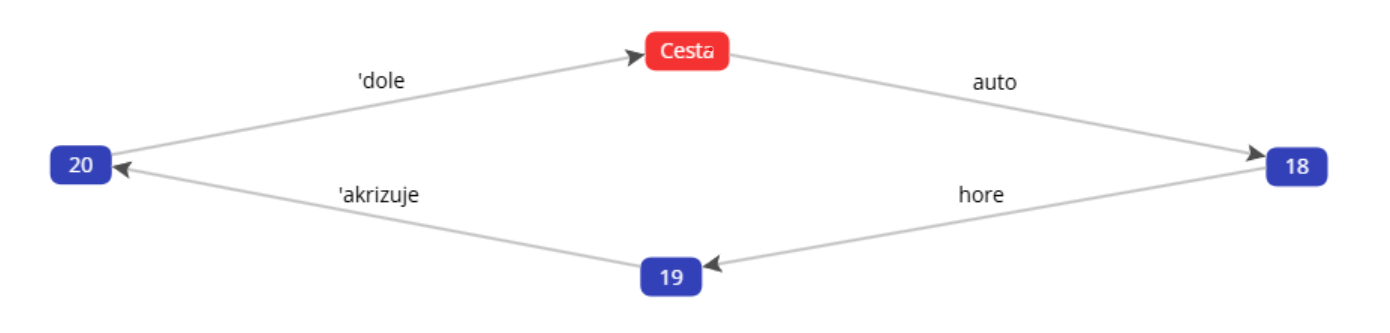
\includegraphics[width=1\textwidth]{cesta.png}
	\caption{Graf procesu Cesta}
\end{figure}

\begin{figure}[!h]
	\centering
	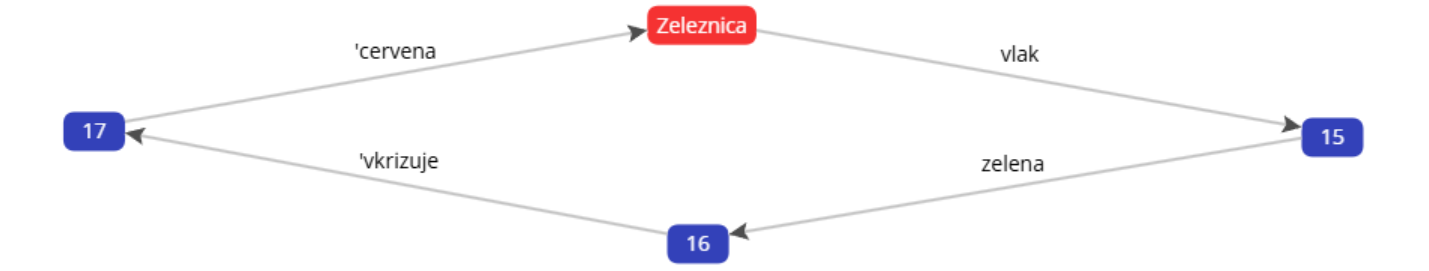
\includegraphics[width=1\textwidth]{zeleznica.png}
	\caption{Graf procesu Železnica}
\end{figure}

\begin{figure}[!h]
	\centering
	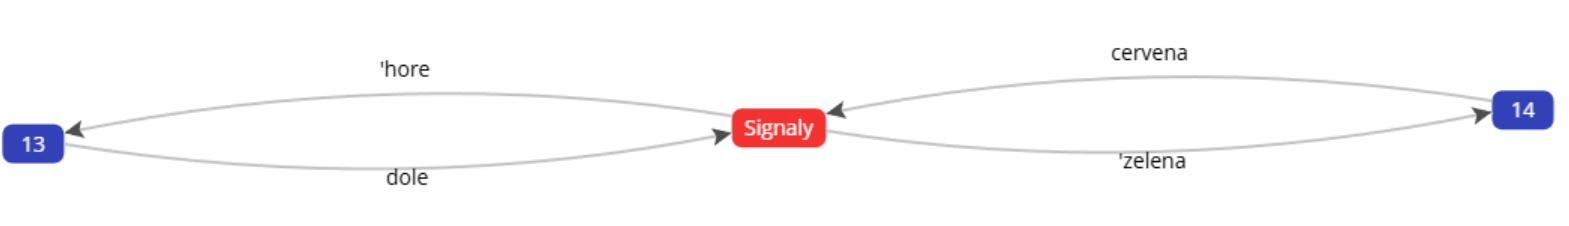
\includegraphics[width=1\textwidth]{signaly.png}
	\caption{Graf procesu Signály}
\end{figure}

Vidíme, to čo by sme očakávali, že procesy Cesta a Železnica sú jednoduché cykly a proces Signály je tvorený dvomi nezávislými cyklami.

\newpage
\section{Graf Priecestia} 

\begin{figure}[!h]
	\centering
	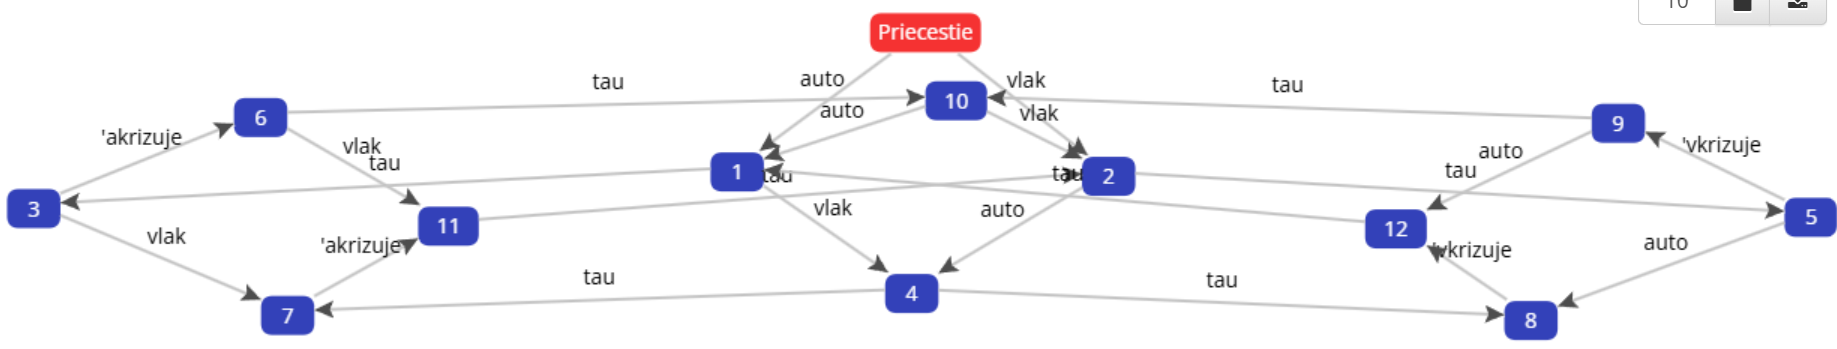
\includegraphics[width=1\textwidth]{priecestie.png}
	\caption{Graf procesu Priecestie}
\end{figure}

Vidíme, že k priecestie môže buď len auto (1), len vlak (2) alebo obe (4). Následne však vidíme, že aj napriek tomu, že pri križovatke môžu byť obe vozidlá respektíve ku križovatke stále môže druhé vozidlo prísť, do križovatky vojde vždy len jedno, na ľavej strane vidíme prípad kedy dostane vlak zelenú a na pravej prípad keď dostane auto horé závory, absencia hrán medzi týmito prípadmi by mala znamenať, že nemôžu nastať súčasne... Asi nie úplne pravda ale aspoň to znie rozumne :P

\end{document}